\documentclass[12pt,a4paper]{article}

\usepackage[margin=0.75in]{geometry}

%Used for doing math things
\usepackage{amsmath}

%Used for fonts, I guess?
\usepackage{amsfonts}

%allows for bold-faced mathematical symbols (like beta)
\usepackage{bm}


%I have no idea what this does, so I commented it out. If the file breaks, try un-commenting this out.
%\usepackage[latin1]{inputenc}

% Amssymb is for assorted symbols
\usepackage{amssymb}

%This allows for the enumeration of
\usepackage{enumitem}

%Used for seting the spacing density. 
\usepackage{setspace}

%The first package is used for incorporating images into the LaTeX file
\usepackage{graphicx}

%Allows the usage of the [H] argument, which forces figure/tabular placement to be HERE and nowhere else. 
\usepackage{float}

%These are useful commands I've hard-coded in.  
\newcommand{\eps}{\epsilon}
\newcommand{\braket}[1]{\left<#1\right>}
\newcommand{\bra}[1]{\left< #1 \right|}
\newcommand{\ket}[1]{\left| #1 \right>}
\newcommand{\comm}[1]{\left[ #1 \right]}
\newcommand{\cross}{\times}
\newcommand{\abs}[1]{\left| #1 \right|}
\newcommand{\bvec}[1]{\bm{#1}}

%rcurs is the basic cursive one
%\def\rcurs{{\mbox{$\resizebox{.16in}{.08in}{\includegraphics{ScriptR}}$}}}
%\def\brcurs{{\mbox{$\resizebox{.16in}{.08in}{\includegraphics{BoldR}}$}}}
%\def\hrcurs{{\mbox{$\hat \brcurs$}}}



%Use this if you use images. Default path is the file's directory. 

%\graphicspath{ {Path} }

\usepackage{cancel}

% Fancy Title

\usepackage{array}
\newcolumntype{P}[1]{>{\centering\arraybackslash}p{#1}}
\newcolumntype{R}[1]{>{\raggedright\arraybackslash}p{#1}}
\newcolumntype{L}[1]{>{\raggedleft\arraybackslash}p{#1}}
\newcommand{\Qbox}[1]{\noindent\fbox{\parbox{\textwidth}{#1}}}

\singlespacing

\begin{document}
\begin{table}
	\centering
	\begin{tabular}{R{2in} P{2in} L{2in}}
		Benjamin Smithers & \begin{tabular}{c}{\Large Systematic Downsizing} \\ {\small with math Daemonflux }  \end{tabular} & Spring 2023 \\\hline
	\end{tabular}

\end{table}

\section{Introduction and Summary}

Here we present a review of a method for treating highly correlated sets of nuisance parameters. In short, one can transform the nuisance parameter basis into one where the parameters are uncorrelated.
Then, we find whih new parameters have the largest effect on ones reconstructed signal, and identify the minimum number that will be necessary to span the space of shapes presentable by the full set of nuisance parameters in your reconstructed space. 

\section{De-correlating systematic uncertainties}\label{sec:decor}

Consider a set of $n$ nuisance parameters $\vec{x}$, each with mean $\mu$.
A $n\times n$ matrix, $\Sigma$ defines the positive-definite covariance between these nuisance parameters. 
If we assume the distribution is jointly normally distributed, then the probability density function defining the odds of sampling a set of nuisance parameters, $\vec{y}$, is given by
\begin{equation}
    P(\vec{y}) = \dfrac{1}{(2\pi)^{n/2}\abs{\Sigma}^{1/2}}\exp\left[-\tfrac{1}{2}(\vec{y}-\vec{\mu})^{T}\Sigma^{-1}\left(\vec{y}-\vec{\mu}\right)\right]
\end{equation}
where $\abs{\Sigma}$ is the determinant of $\Sigma$. We can first consider the transformation 
\begin{equation}
    \vec{p}\equiv \vec{y}-\vec{\mu}
\end{equation}
and consider instead the \textit{log} of the likelihood.
This allows us to drop off the prefactors, since we ultimately will only care about the differences in log likelihoods.
What we then have is 
\begin{equation}
    \ln P \equiv LLH \sim -\tfrac{1}{2}\vec{p}^{T}\Sigma^{-1}\vec{p}
\end{equation}
We can now, by construction, define a transformation $U$, satisfying $UU^{T}=I$, and a diagonal matrix $A$ such that 
\begin{align}\label{eq:combo}
    A&=U\Sigma^{-1}U^{T} & LLH &\sim -\tfrac{1}{2}(U\vec{p})^{T} U\Sigma^{-1}U^{T}(U \vec{p})
\end{align}
and we recover
\begin{equation}
    LLH \sim -\tfrac{1}{2}\vec{p'}^{T} A\vec{p'},
\end{equation}
where the primed vectors refer to the vectors transformed by $U$. The left side of equation~\eqref{eq:combo} can be re-expressed as 
\begin{align}
    A&=U\Sigma^{-1}U^{T} &  &\to & A' &= U^{T}\Sigma U,
\end{align}
or, since $A$ is diagonal,
\begin{equation}\label{eq:mat}
\Sigma U = U\left[ \begin{array}{cccc}\lambda_{!} & 0 & \ldots & 0 \\
0 & \lambda_{2} & \ldots & 0 \\
\vdots & \vdots & \ddots & \vdots \\
0 & 0 & \ldots & \lambda_{n} \end{array}\right].
\end{equation}
If we re-write the transformation matrix $U$ as a vector of its column vectors $\eta_{i}$, $U=\left[\begin{array}{ccc}\eta_{1} & \ldots & \eta_{n} \end{array}\right]$ then Equation can be expressed as 
\begin{equation}
\Sigma \eta_{i} = \lambda_{i}\eta_{i}.
\end{equation}
This tells us that the column vectors of the transformation matrix $U$ are the right eigenvectors of the covariance matrix $\Sigma$. 
And each of the corresponding eigenvalues of $\Sigma$ are the entries along the diagonals in $A'$.

So, for a given covariance matrix $\Sigma$, we solve for its eigenvalues and eigenvectors. 
The eigenvalues each represent a gaussian prior width for new, uncorrelated, parameters in the new basis. 
The matrix of the eigenvectors allows for transformations from the correlated to the uncorrelated basis. 
Similarly, the inverse of that eigenvector matrix facilitates transformations back from the uncorrelated basis to the correlated basis. 

\section{Ranking}
 
Moving forwards, we need a function that takes a set of correlated nuisance parameters $\vec{x}$ and calculates a binned expectation.
Generally this is done in three steps
\begin{enumerate}
    \item Generate a Monte Carlo sample
    \item Use the Monte Carlo sample to calculate a binned central expectation for your sample
    \item For each parameter $i$, and for each event $j$, calculate the 1D gradient for the weight about the central expectation, $\left.\tfrac{\partial w_{j}}{\partial x_{i}}\right|_{central}$
\end{enumerate}
Then each parameter could in principle be perturbed independently, a new weight calculated for each simulated event, and a new overall expectation calculated. Since the nuisance parameters are correlated, this isn't a good idea.  

Using the methods of Section~\ref{sec:decor}, we solve for the eigenvalues and vectors of the covariance matrix to determine the transformation to the un-correlated basis and the widths of the uncorrelated priors. 
For each uncorrelated parameter, we transform its $1\sigma$ deviation from its central value into the correlated basis, and use this set of nuisance parameters to calculate an expectation from the Monte Carlo gradients. 

We can then use a likelihood function, such as Equation\ref{eq:llh}, to calculate the impact of the uncorrelated parameter.
\begin{equation}\label{eq:llh}
-\Delta LLH = \tfrac{1}{2}\sum_{i=0}^{bins} \left(\dfrac{p_{i}-\mu_{i}}{\sigma_{i}}\right)^{2},
\end{equation}
summing over the $i$ bins, where $p_{i}$ is the perturbed value in a bin, $\mu$ is its mean, and $\sigma$ is the expected variance in the bin. For a Poissonian error, $\sigma=\sqrt{\mu}$.  

\section{Trimming}

\section{Daemonflux}

Daemonflux~REF is combines the uncertainties on both the overall cosmic ray flux and the hadronic production rates in the cosmic ray air showers that follow when they impact our atmosphere.
It is comprised of six ``global spline fit" parameters and seventeen more that relate to pion and kaon production at various energies. 
These parameters are highly correlated, as shown in Figure~\ref{fig:cov}. 
\begin{figure}\label{fig:cov}
    \centering
    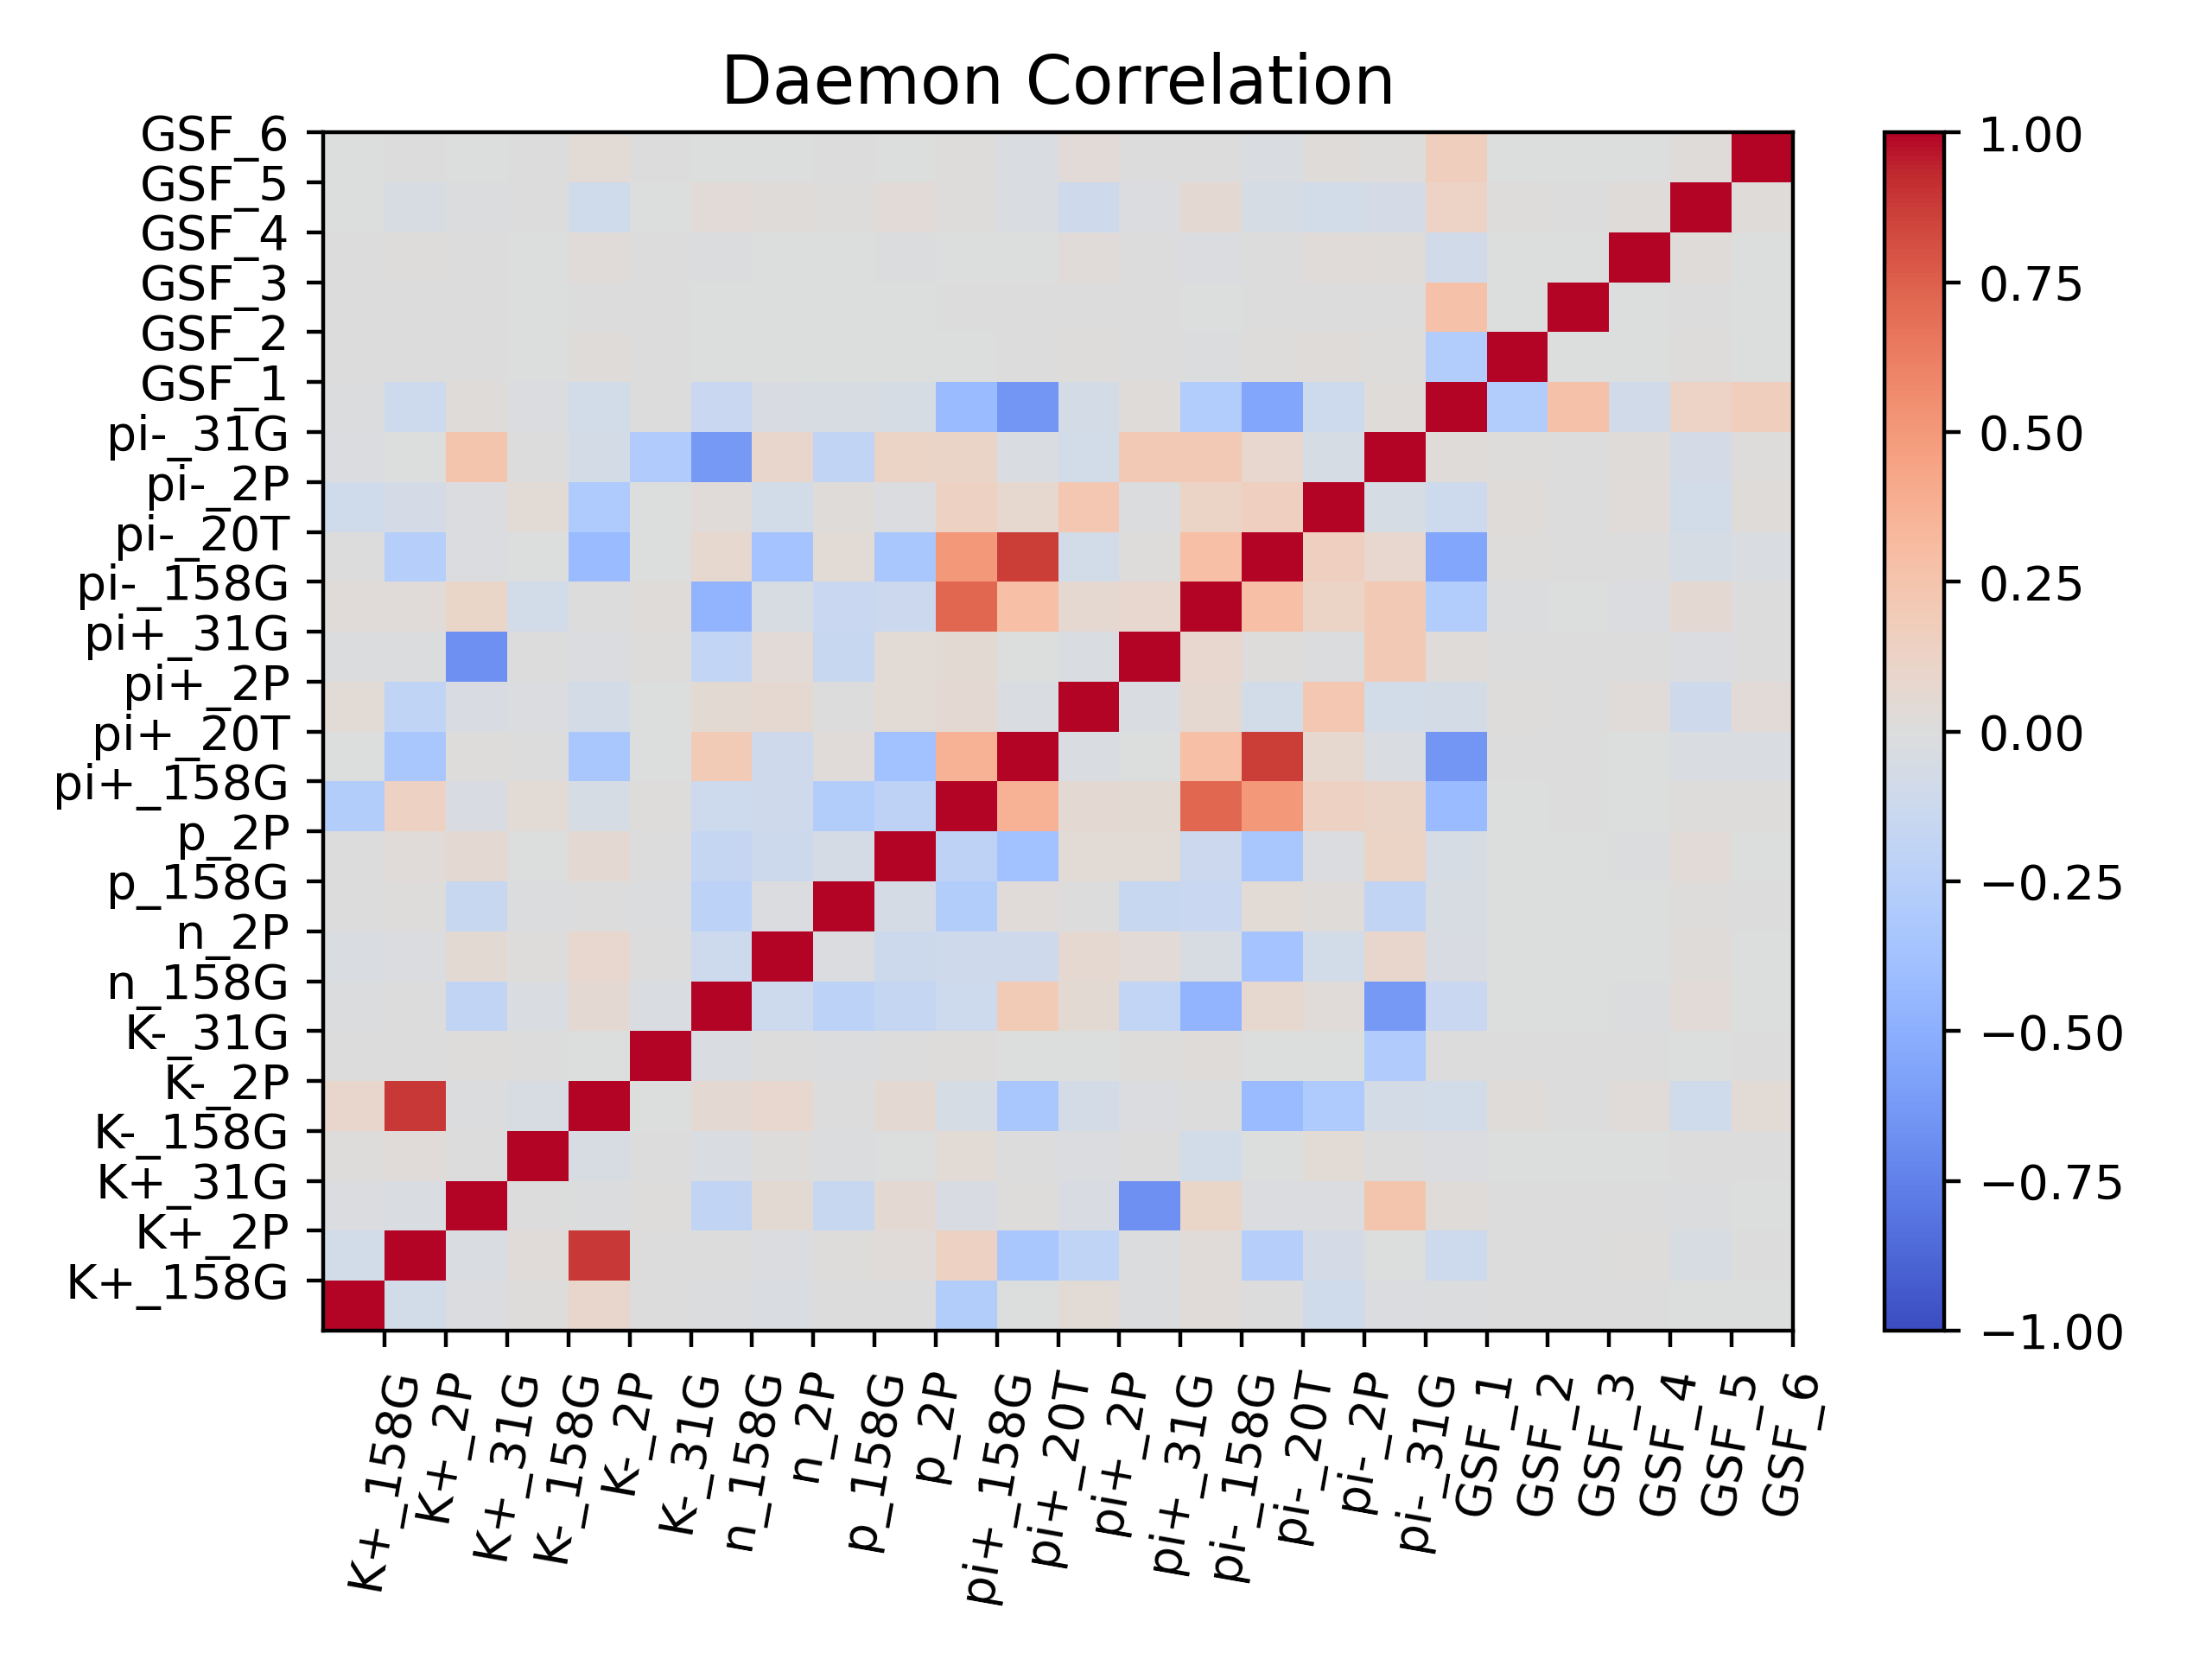
\includegraphics[width=0.75\linewidth]{./figures/daemon_cov.png}
\end{figure}

Write about the gradient extraciton. 

We proceed with calculating a new basis as in the previous sections, and calculate the impact of the new orthogonal parameters.
This is done for the cascades sample developed by the diffuse group, and used in ongoing MEOWS analyses\footnote{MEOWS-C-2023}. 
These are shown in Figure~\ref{fig:impact}.
\begin{figure}\label{fig:impact}
    \centering
    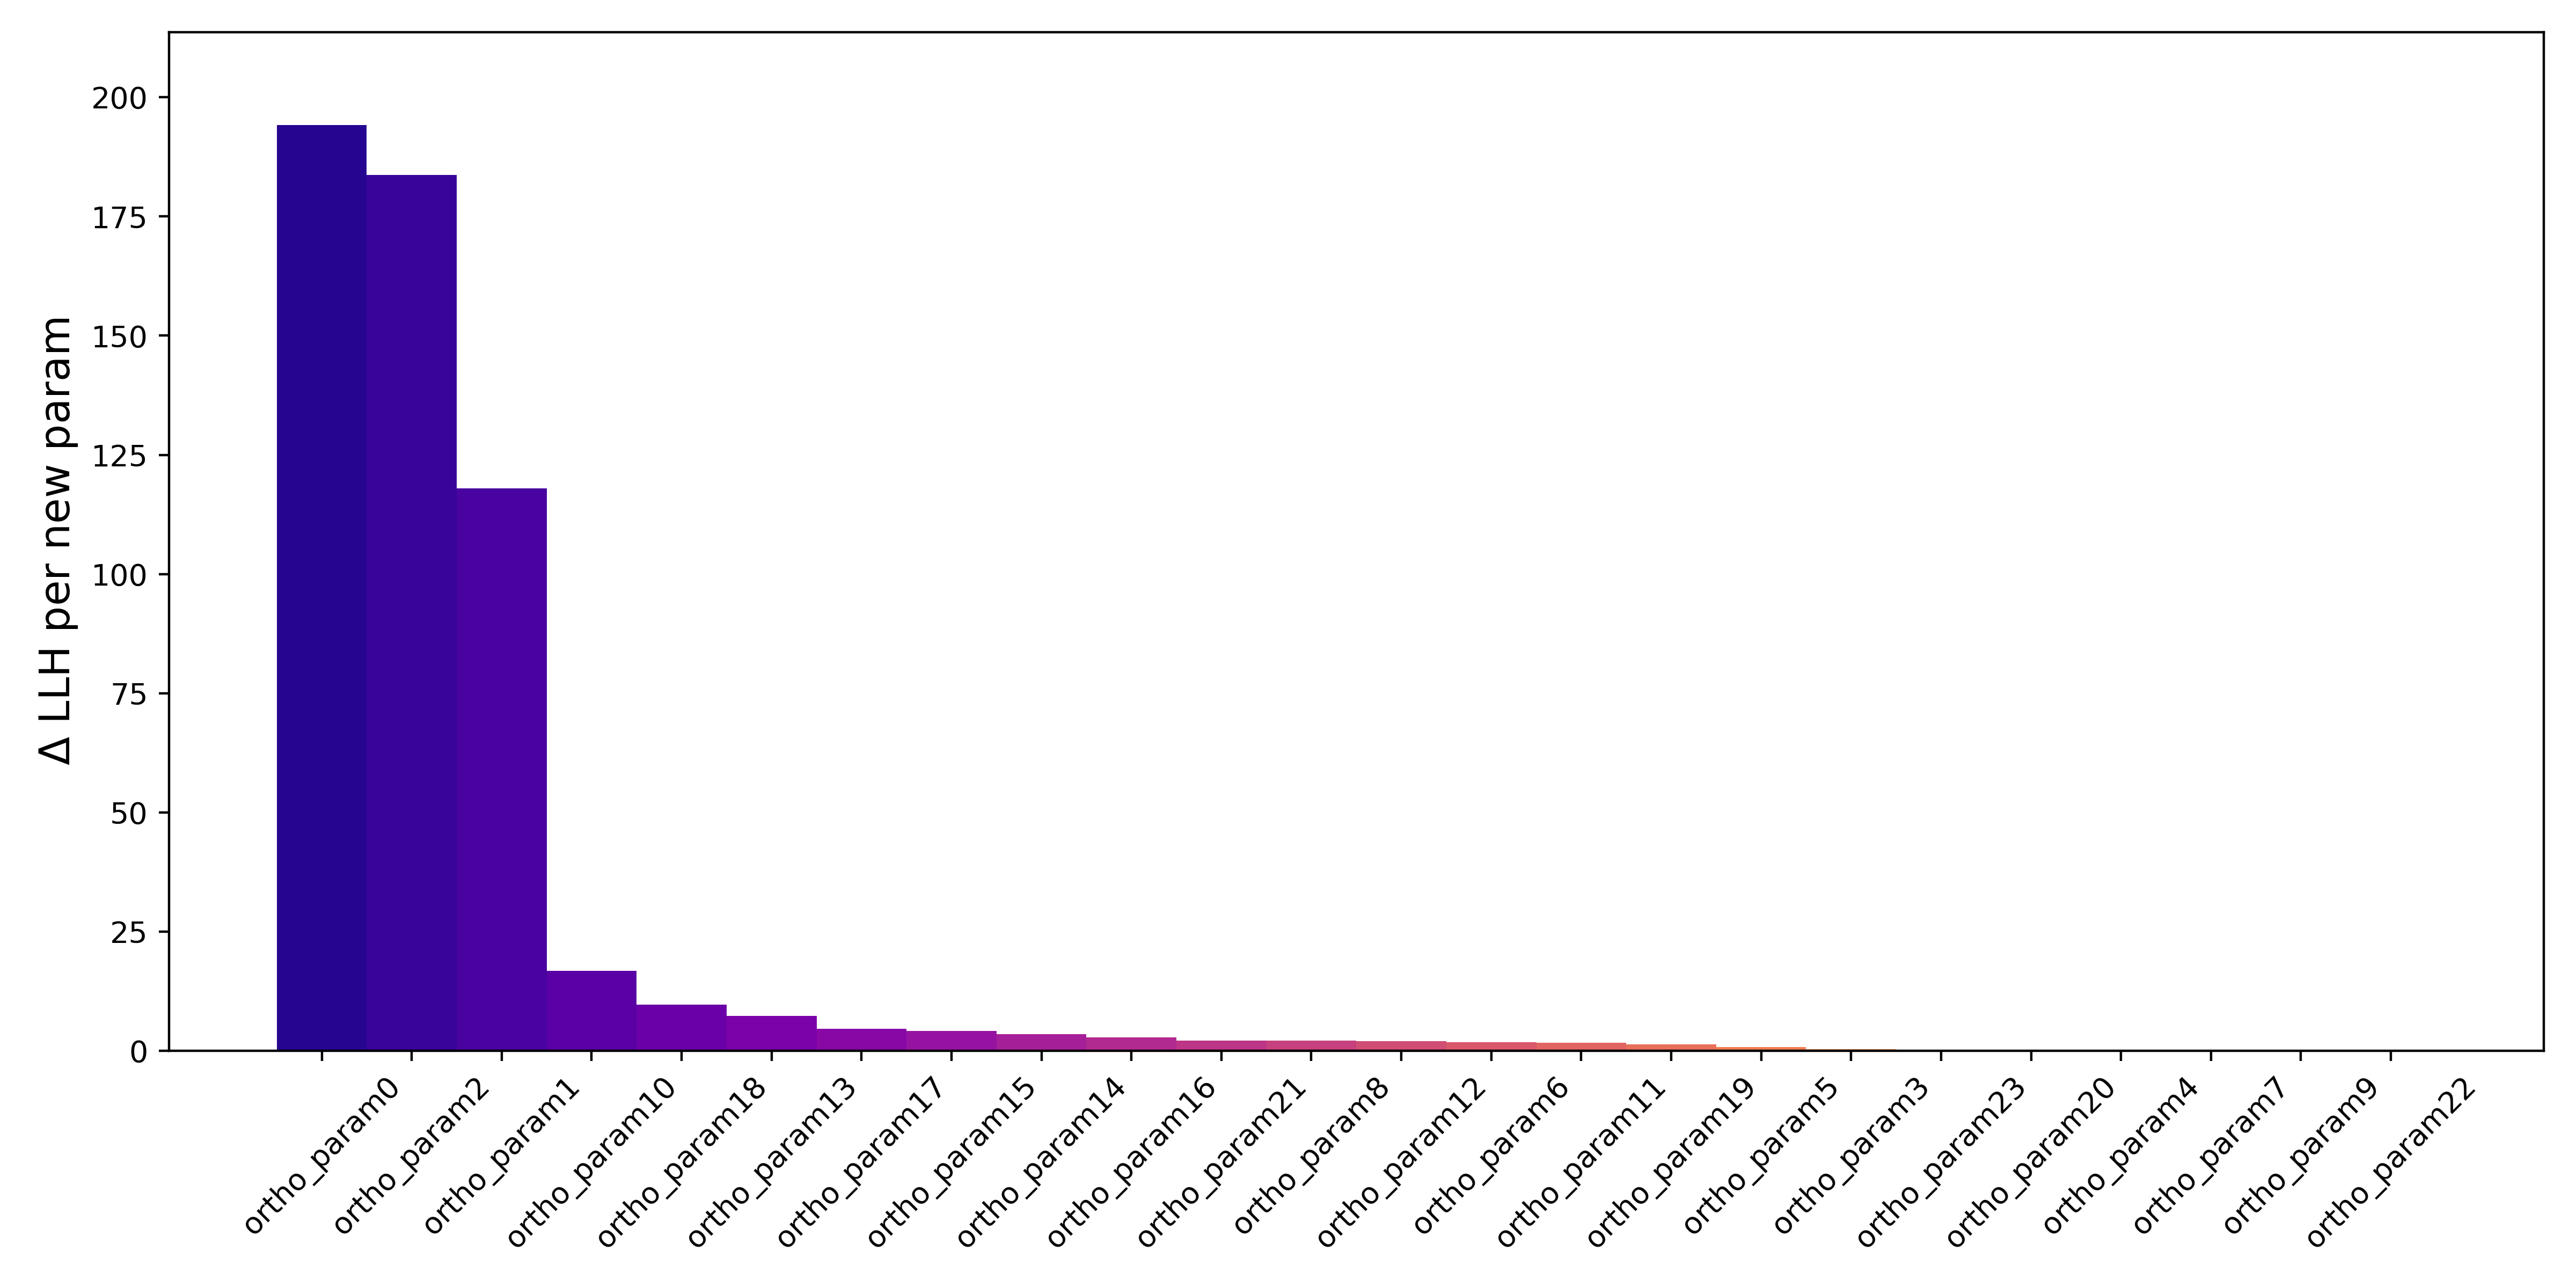
\includegraphics[width=0.75\linewidth]{figures/daemon_distr.png}
\end{figure}
As is evident, the first few parameters have a much greater impact than those that follow.

\subsection{Variance Testing}

We first allow only the parameter with the biggest pull to vary, or ``ortho\_param0". 
We then sample this value 10,000 times and calculate the $\Delta LLH$ at each sample. 
We note the threshold value of $\Delta LLH$ below which 90\% of the samples $\Delta LLH$'s lie. 
This process is then repeated for the two parameters with the largest pulls, and the new threshold noted.
This is repeated until all 23 parameters are being varied at each step. 
The $\Delta LLH$ thresholds, normalized to the one varrying the most, are shown in Figure~\ref{fig:distr}, where a horizontal line has been drawn at 0.95. 
\begin{figure}\label{fig:distr}
    \centering
    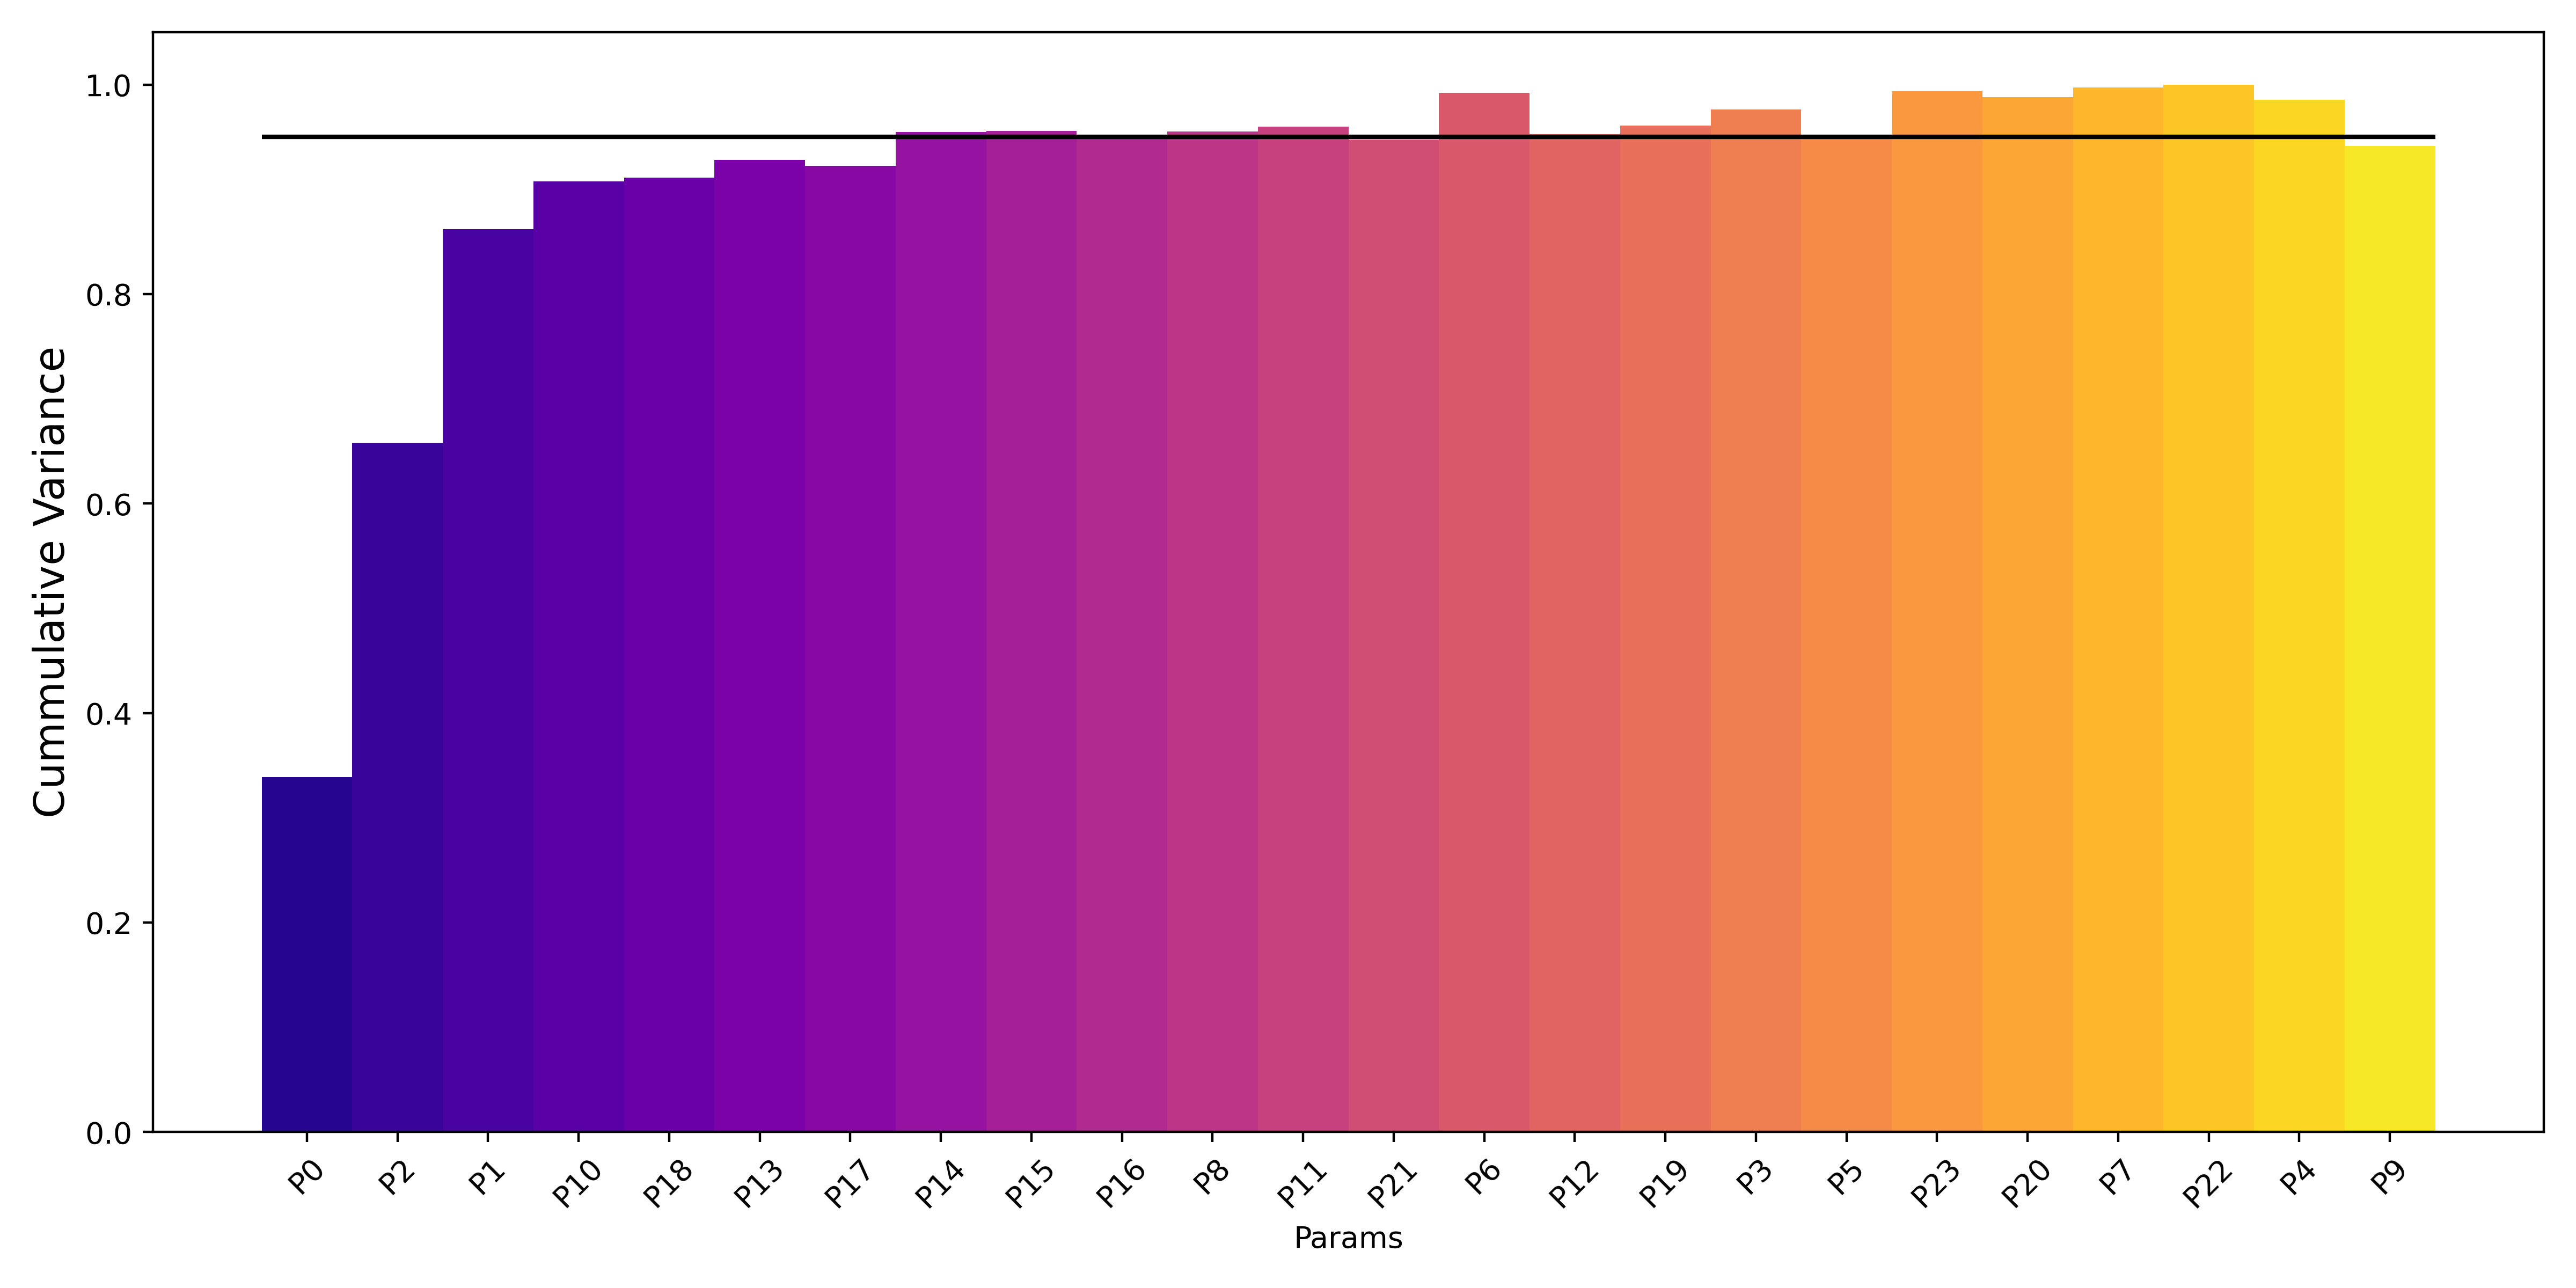
\includegraphics[width=0.8\linewidth]{./figures/daemon_variance_cummulative.png}
\end{figure}
From this figure, we gather that seven or eight parameters are needed to account for 95\% of the variance in the whole ensemble. 

\subsection{Shape Testing}

It is also important to ensure the full configuration of shapes achievable, in reconstructed space, with a 23 parameter ensemble is also possible to achieve with a reduced number of parameters. 
To test this, we sample all 23 parameters randomly. Then, by allowing only the $m$ strongest pulling parameters to vary, we carry out a fit to the fully shuffled expectation while leaving the last $23-m$ parameters fixed at their central values. 
The distributions of best-fit $\Delta LLH$, are shown in Figure~\ref{fig:res}.
\begin{figure}\label{fig:res}
    \centering
    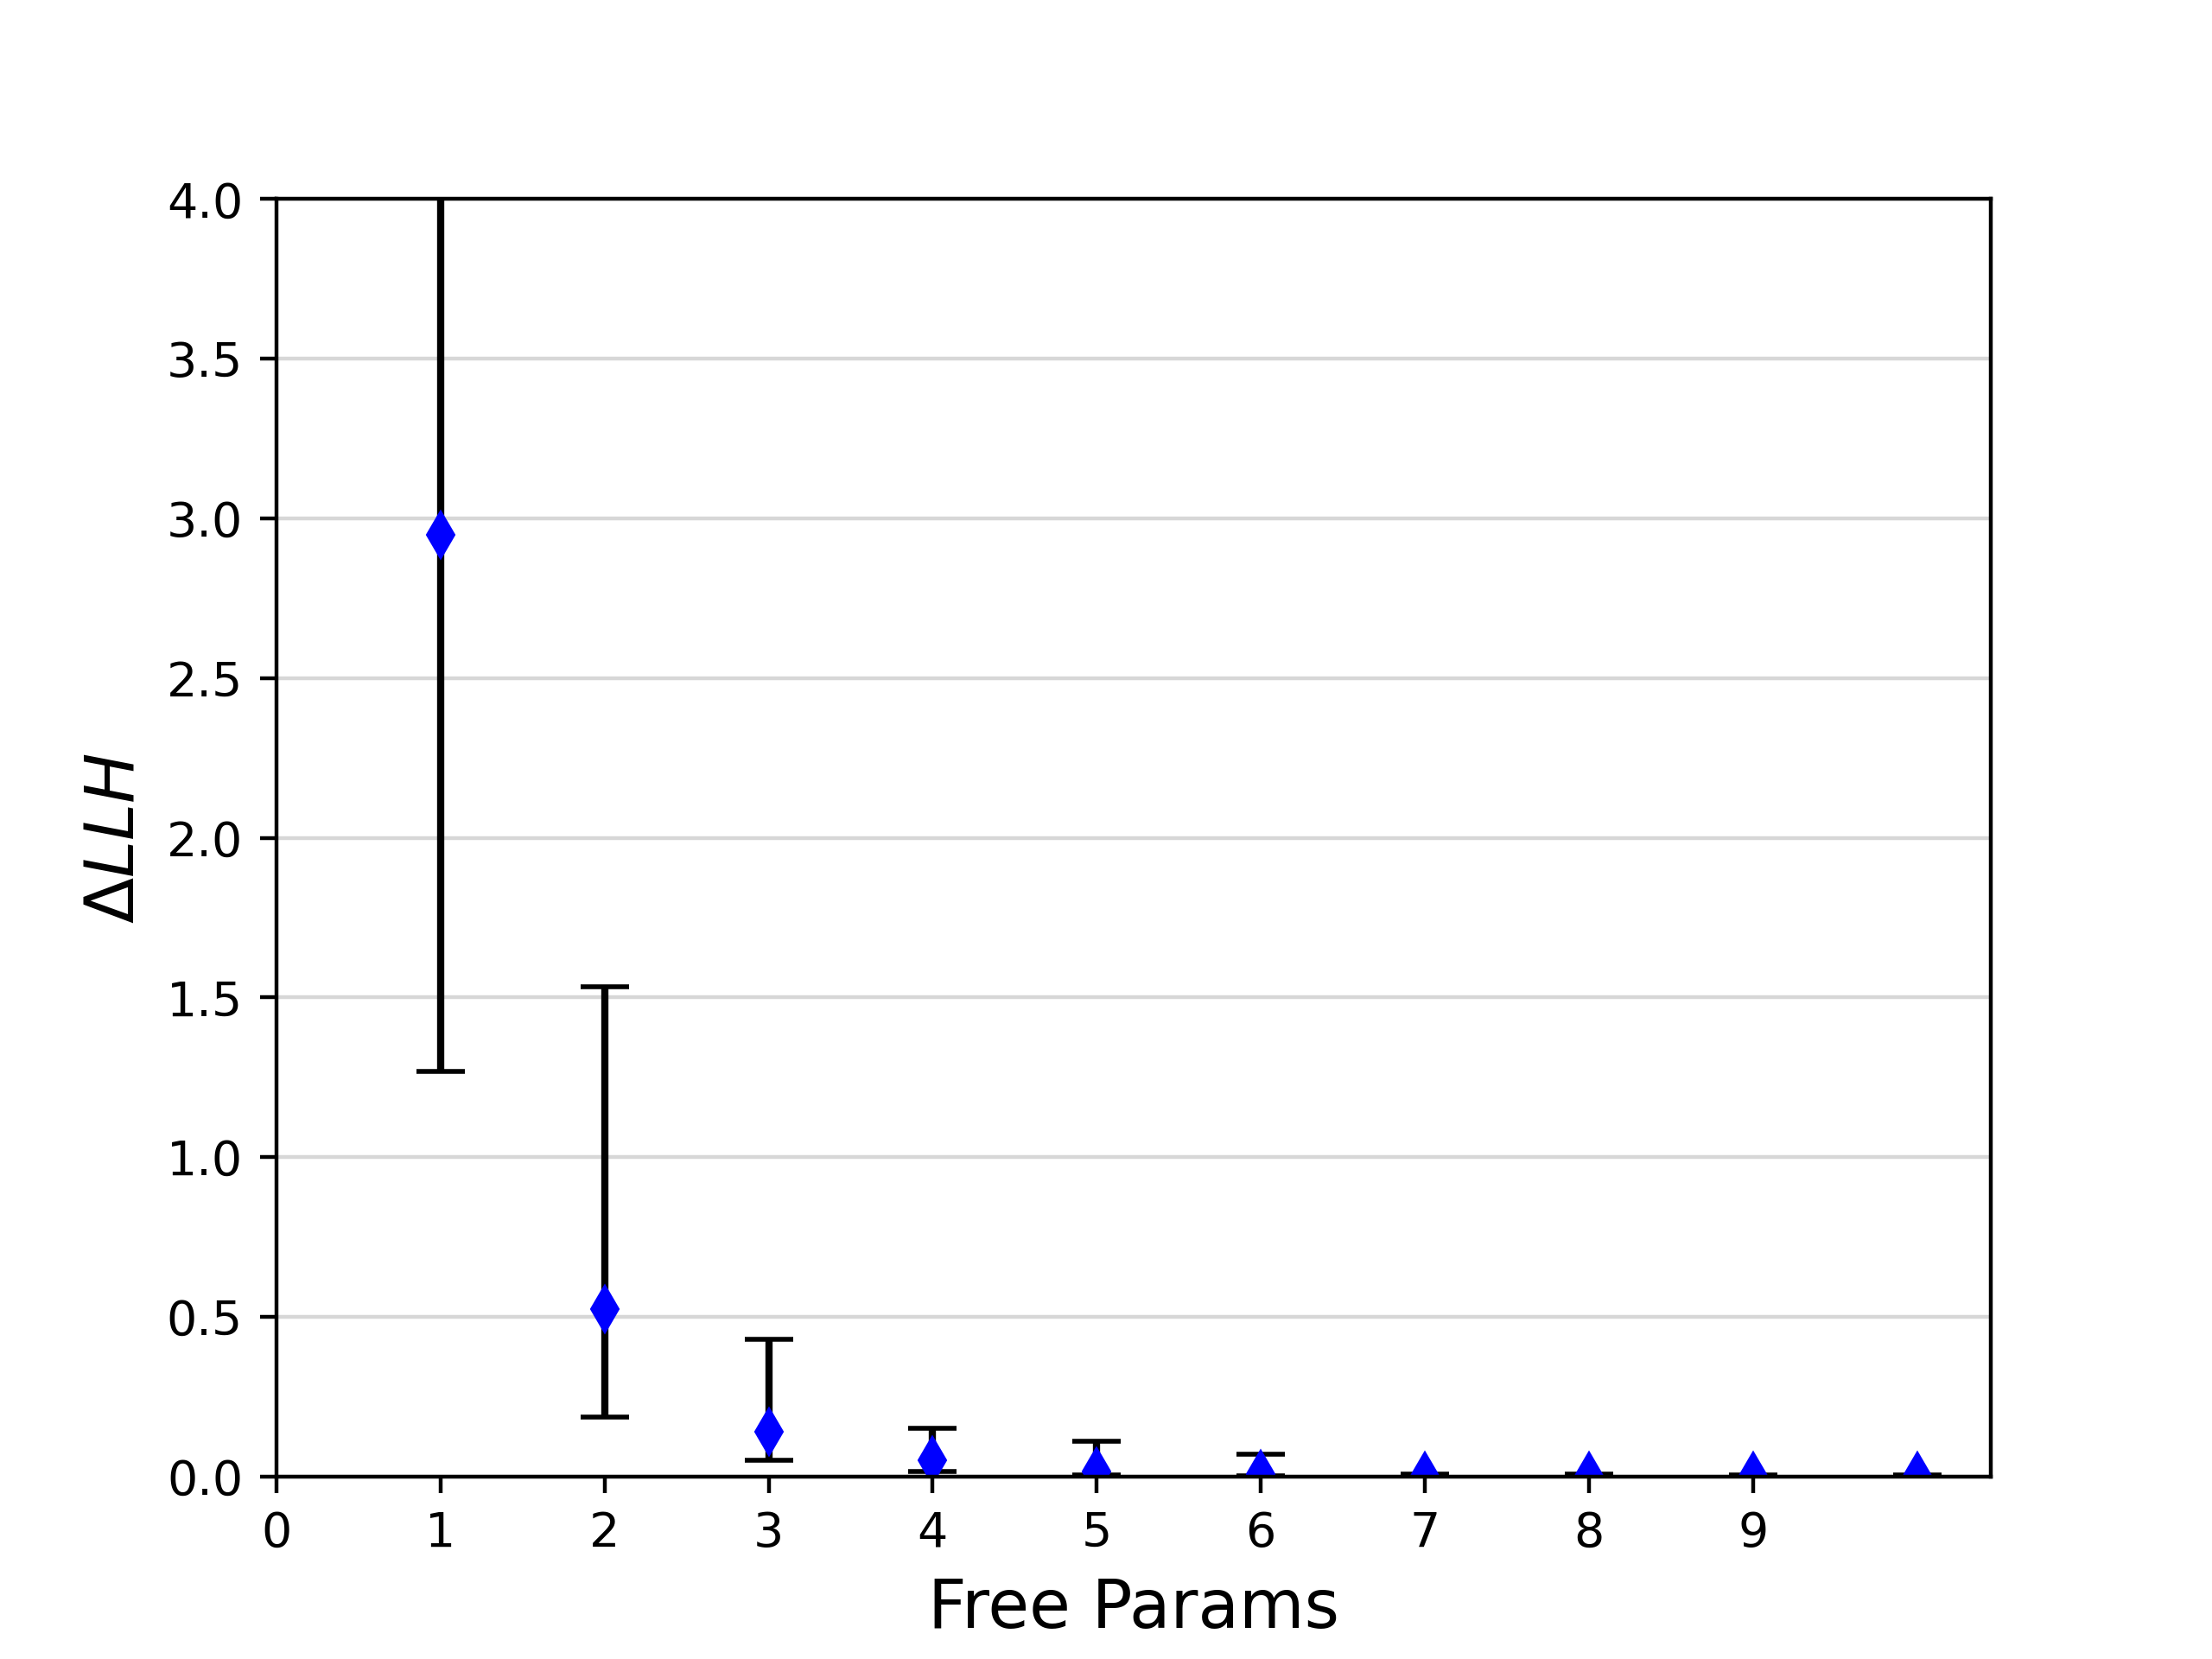
\includegraphics[width=0.75\linewidth]{./figures/results.png}
\end{figure}
From this, most shapes appear to be realizable with as few as five parameters, although with some occasional deviations. 
Once seven parameters are allowed to vary, no discrepancies are observed between fits and expectations generated with a full 23-parameter sampling. 


\end{document}